\documentclass[../portafolio.tex]{subfiles}



\begin{document}

\section{Números aleatorios} 

\hfill \textbf{Fecha de la actividad:} 18 de noviembre de 2022

\medskip


%-----------------------------------------------------%
%-----------------------------------------------------%
%-----------------------------------------------------%

\subsection{Objetivo de la clase}

En este laboratorio se trabajó con números aleatorios para encontrar el número $\pi$, para ello se utilizó la función \texttt{numpy.random.rand(N)} que retornaba N números aleatorios ubicados en el intervalo $]0,1[$.

\vspace{2mm}
En este laboratorio trabajé junto a Eduardo Escudero y Jeremías Martínez.



%-----------------------------------------------------%
%-----------------------------------------------------%
%-----------------------------------------------------%

\subsection{Desarrollo del laboratorio}

Se trabajó creando una circunferencia inscrita en un cuadrado de lado 1 con el fin de relacionar de forma analítica el área del cuadrado con el de la circunferencia y de forma numérica encontrar el valor de $\pi$. 

\vspace{2mm}
El área de una circunferencia es $A_{circunf}= \pi r^2$ y el de un cuadrado de lado $2r$ es $A_{cuad}=4r^2$, al relacionarlo se obtiene la ecuación \ref{ec_pi}.

\begin{equation}
    4 \frac{A_{circunf}}{A_{cuad}} = \pi  \label{ec_pi}
\end{equation}

Ahora, si se toman en cuenta la cantidad de puntos que se encuentran dentro de un cuadrado de lado $2r$ y la cantidad de puntos que se encuentran dentro de una circunferencia de radio $r$ inscrita en el cuadrado, entonces al relacionar la cantidad de puntos que se encuentran dentro de las figuras, como si fueran el área de ellas, se debería cumplir la relación expuesta en la ecuación \ref{ec_pi}.

\vspace{2mm}
Para encontrar el número $\pi$ se comenzó creando el código \ref{C1-aleatorio}. En las líneas 1 y 2 del código se generaron $N =20000$ números aleatorios entre $]0,1[$ para los valores de $x$ y para los valores de $y$, luego, en la línea 4 y 5 se crearon la misma cantidad de números aleatorios entre el intervalo $]-1,0[$ para $mx$ y $my$. Seguidamente, en la línea 7 se concatenaron los \texttt{arrays} $mx$, $x$, $mx$ y $x$ y en la línea 8 se concatenaron los \texttt{arrays} $my$, $y$, $y$ e $my$, y se dividieron por 2, de este modo, se obtuvo que $xx$ e $yy$ correspondían a 80000 números aleatorios entre $]-0.5,0.5[$. Finalmente se graficó $yy$ con respecto a $xx$ generando un cuadrado de lado 1 con centro en el origen. 
  

\begin{listing}[h]
    \begin{minted}[
frame=lines,
framesep=2mm,
baselinestretch=1.2,
bgcolor=LightGray,
fontsize=\footnotesize,
linenos
]
{python}
x=np.random.rand(int(N))
y=np.random.rand(int(N))

mx=-np.random.rand(int(N))
my=-np.random.rand(int(N))

xx=np.concatenate( [ mx,x,mx,x] ) /2
yy=np.concatenate( [ my,y,y,my] ) /2
    \end{minted}
\caption{Fragmento de código que crea dos \texttt{arrays} de N números aleatorios en el intervalo $]-0.5,0,5[$}
\label{C1-aleatorio}
\end{listing}


\vspace{2mm}
Luego, el código \ref{C2-aleatorio} se ocupó para encontrar que valores de $xx$ y de $yy$ se encontraban dentro de la circunferencia inscrita dentro del cuadrado de lado 1 centrado en el origen. Con la ayuda de un ciclo \texttt{for} en la línea 4 se encontró la distancia de los puntos con respecto al origen, si la distancia era menor que $0.5$ entonces los valores se añadían a la lista $xa$ y $ya$. En el gráfico \ref{aleatorio_circunf} se puede apreciar una circunferencia de radio $0.5$ con centro en el origen, este se consiguió graficando $ya$ con respecto a $xa$ obtenidos en la línea 7 y 8 del código \ref{C2-aleatorio}. 





\begin{listing}[h]
    \begin{minted}[
frame=lines,
framesep=2mm,
baselinestretch=1.2,
bgcolor=LightGray,
fontsize=\footnotesize,
linenos
]
{python}
xa= []
ya= []
for n in range(len(xx)):
    r = np.sqrt(xx[n]**2 + yy[n]**2)

    if r<0.5:
        xa.append(xx[n])
        ya.append(yy[n])
    \end{minted}
\caption{Fragmento de código que crea una lista con los valores que se encuentran dentro de una circunferencia de radio $0.5$ centrada en el origen. }
\label{C2-aleatorio}
\end{listing}


\begin{figure}[h]
    \centering
    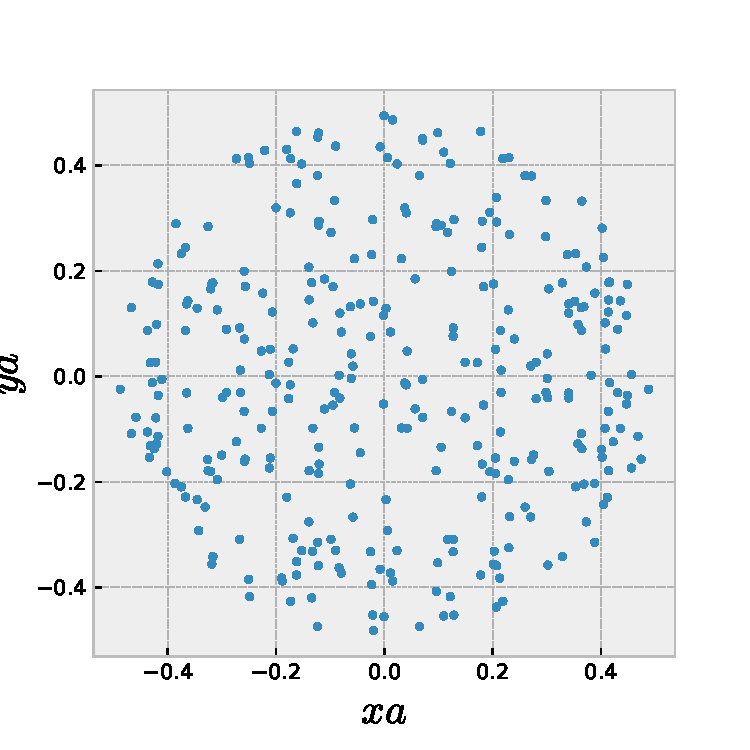
\includegraphics[scale=0.8]{tex/img/circunf_pi.pdf}
    \caption{ 100 números generados aleatoriamente dentro de una circunferencia de radio $0.5$.}
    \label{aleatorio_circunf}
\end{figure}

\vspace{2mm}
Con la circunferencia ya encontrada se procedió a calcular el valor de $\pi$, para ello, siguiendo la ecuación \ref{ec_pi}, se dividieron todos los punto que se encontraban dentro de la circunferencia, es decir, el tamaño de $xa$ con todos los puntos que se encontraban dentro del cuadrado, es decir, $4N=80000$ y el resultado se multiplicó por 4. De este modo, se obtuvo que $\pi \approx 3.1424$.

\vspace{2mm}
Para observar cómo variaba el valor de $\pi$ con respecto al número de valores generados aleatoriamente se creó que gráfico \ref{puntos_pi}. En el eje $x$ de este gráfico se muestra la cantidad de números generados y el eje $y$ representa el valor que toma $\pi$. En resumen, se puede decir que mientras mayor sea la cantidad de números generados aleatoriamente el valor obtenido al resolver la ecuación \ref{ec_pi}, en general, tenderá al valor real de $\pi$. 




\begin{figure}[H]
    \centering
    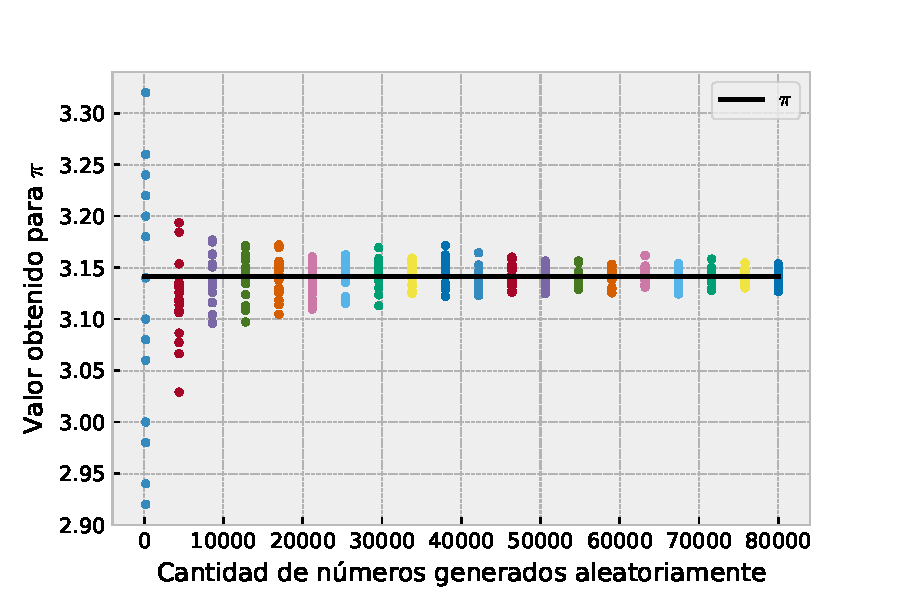
\includegraphics[scale=0.8]{tex/img/puntos_pi.pdf}
    \caption{Este gráfico relaciona la cantidad de números generados aleatoriamente con el valor obtenido para $\pi$, además está graficada una recta que indica el valor real de $\pi$}
    \label{puntos_pi}
\end{figure}









%-----------------------------------------------------%
%-----------------------------------------------------%
%-----------------------------------------------------%

\subsection{Conclusiones}
En este laboratorio se trabajó con números aleatorios, ocupándolos para encontrar el número $\pi$. Primero se crearon número aleatorios del $]-0.5\,0.5[$ para el eje $x$ y para el eje $y$, luego se graficaron obteniéndose de esta manera un cuadrado de largo $1$ con centro en el origen. Después se separaron los puntos generados aleatoriamente que se encontraban dentro de una circunferencia de radio $0.5$ inscrita dentro del cuadrado y a través de un relación analítica de sus áreas, se encontró un valor aproximado de $\pi$. Finalmente se concluyó que mientras mayor era la cantidad de números generados aleatoriamente, entonces la aproximación al número $\pi$ sería mejor.

\vspace{2mm}
En este laboratorio aprendí a que los números aleatorios pueden ser útiles para trabajar con métodos numéricos como lo fue en este caso encontrando el número $\pi$. También aprendí que los números aleatorios generados por un computador no son realmente aleatorios y que nunca lo serán, pues necesitarán de todos algún algoritmo que los genere.

\vspace{2mm}
Por otra parte, me hubiese gustado trabajar un poco más en crear números aleatorios, quizás creando alguna función más compleja que se asemejara a \texttt{numpy.random.rand()}.


\end{document}